\chapter{Estudio del Problema Singular}

En este capitulo se van a aplicar las herramientas desarrolladas en el capitulo anterior al estudio del espectro de un operador singular.

\section{El Operador Singular}

Como trabajo de tesis se propondrá aplicar los métodos desarrollados en el capitulo anterior al operador diferencial (\ref{operador}).

\begin{equation}
\begin{array}{c}
    A \phi (x) = - \partial ^2 _x  \phi(x) + \frac{\alpha}{x} \phi(x) \\[5pt]
    \phi(0) = \phi(L) = 0 
\end{array}
\label{operador}
\end{equation}

Para eso voy a resolver la ecuación de autovalores (\ref{eq.aut.sin}).

\begin{equation}
\begin{array}{c}
    A  \phi (x)  =   \lambda ^2 \phi (x) \\[5pt]
    \lambda \ \in \ \mathfrak{R} _+
\end{array}
\label{eq.aut.sin}
\end{equation}




La cual posee soluciones LI, $ y_1 $ y $ y_2 $ dadas por :

\begin{equation}
    \phi (x) = 
    C[1]
    \underbrace{
     \ e ^{-i \lambda x} \ x \ F _{1} ^{1} (1+\frac{ \alpha}{2 \lambda i },2,2 i \lambda x) } _ {y_1}
    + C[2] \underbrace{ \ e^{-i \lambda x } \ x \ U (1+\frac{ \alpha}{2 \lambda i },2,2 i \lambda x) } _{y_2} 
\label{eq.phi}
\end{equation}




Donde $F _1 ^1(a,b,z)$ y $ U(a,b,z)$ son las soluciones LI de la ecuación hypergeométrica:

\begin{equation}
    z \ \partial ^2 _z \ \psi (a,b,z) + (b-z) \
    \partial _z \psi (a,b,z)
    -a \ \psi (a,b,z) = 0
\end{equation}

Las cuales poseen las expresiones analíticas  : 

\begin{equation}
\begin{aligned}
	U(a,b,z) &= \frac{1}{\Gamma (a)} 
	\int _0 ^{\infty} e ^{-zt}
	t ^{a-1}
	(1+t) ^{b-a-1}
	dt \\[5pt]
	F _1 ^1 (a,b,z) &= \sum _ {k=0} ^{\infty} 
	\frac{(a) _k}{(b) _k} 
	\frac{z ^k}{k!} 
\end{aligned}
\end{equation}

Donde $( \   ) _n$ es el símbolo de Pochhammer. \\



\textbf{Espectro del operador:} \\


Para aplicar la condición de contorno $\phi (0) = 0$, hay que hacer un desarrollo de $\phi(x)$  alrededor de $x \rightarrow 0$:

\begin{equation}
\begin{array}{c}
\phi (x \rightarrow 0) \approx
C[1] ( x + O(x ^2)) + 
C[2] x 
\left( 
\frac{1}{  \alpha x  \Gamma ( \frac{ \alpha}{2 i \lambda}  )   }  +
\frac{Ln(x) }{\Gamma ( \frac{ \alpha}{2 i \lambda} ) } + Cte + O(x)
\right)
\\[15pt]
Donde,  \ Cte = 
\frac{
-1 + 2 \gamma + Ln[2 i \lambda] + \psi (1 + \frac{ \alpha}{2 i \lambda})
}
{\Gamma (\frac{i \alpha}{2 \lambda})}
\end{array}
\label{eq.scat}
\end{equation}

Donde se ve que $y _1 (x \rightarrow 0 ) \rightarrow 0$, e $y _2 (x \rightarrow 0)  \rightarrow
\frac{1}{  \alpha   \Gamma ( \frac{i \alpha}{2 \lambda}  )   } $ , entonces la forma de satisfacer la condición de contorno es imponiendo C[2] = 0

Los autovalores estarán dados entonces por los ceros de $y_1 (x= L)$, como el único termino que se anula en el producto es la función Hypergeométrica, los autovalores vienen dados por los ceros de la ecuación:.


\begin{equation}
F _1 ^1 (1+\frac{ \alpha}{2 i \lambda},2,2 i \lambda L)  = 0
\label{eq.1}
\end{equation}

En la figura (\ref{fig:funcion}) se puede observar el comportamiento  de $ | F _1 ^1 (1+\frac{ \alpha}{2 i \lambda},2,2 i \lambda L) | ^2 $ para   $\alpha=1, \ L=1$. \\

\begin{figure}[h!]
\centering
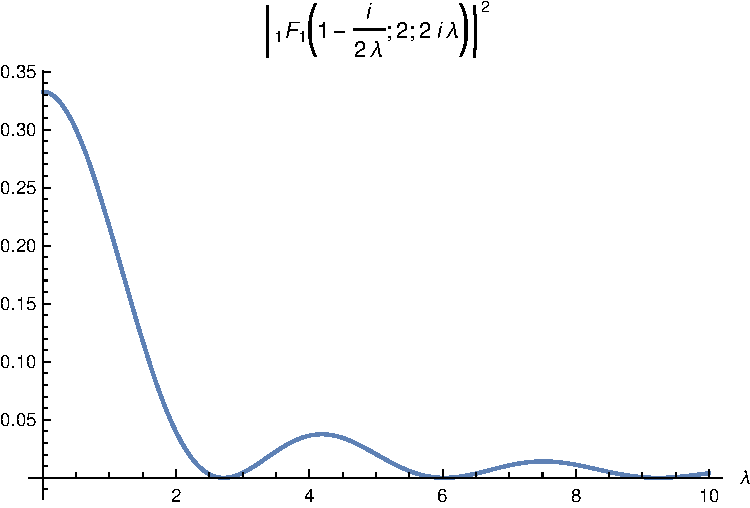
\includegraphics[scale=0.7]{Funcion.pdf}
\caption{En esta imagen se puede ver el comportamiento de los ceros de función $F _1 ^1$, para $\alpha=1$ y $L=1$}
\label{fig:funcion}
\end{figure}

\textbf{Desarrollo en serie:} \\

Para estudiar el espectro de $F _1 ^1$ voy a hacer un desarrollo asintótico alrededor de $\lambda \rightarrow \infty$, el cual está dado por (\ref{eq.aprox})


\begin{equation}
\begin{aligned}
    F _1 ^1 (a,b,z) &= \Gamma (b) 
    \left(
    \frac{e^z z ^{a-b} }{\Gamma(a)} * S_1 + \frac{(-z) ^{ -a}}{ \Gamma(b-a)} 
    * S_2
    \right) \\[5pt]
    S _1 &= \sum _{n=0} ^{\infty} \frac{(b-a) _n (1-a) _n}{n!} z ^{-n} \\[5pt]
    S _2 &= \sum _{n=0} ^{\infty} \frac{(a) _n (1+a-b) _n}{n!} (-z) ^{-n} 
\end{aligned}
\label{eq.aprox}
\end{equation}

$A_1$ y $A _2$ son las correcciones al orden dominante, para calcular el polo de la función $\zeta _A (s)$ en $s=-1/2$ basta tomar $A _1 = A _2 = 1$, que es lo que se hará, luego se trabajará con el desarrollo en serie completo para estudiar los polos mas allá de $s=-1/2$. 



El orden dominante de (\ref{eq.aprox}) es:

\begin{equation}
\begin{aligned}
    F _1 ^1 (1+  \frac{  \alpha}{2 i \lambda} ,2 ,2 i \lambda L  ) & \approx 
    i  \frac{e ^{ \frac{\pi}{4} \frac{\alpha}{\lambda} } }{2 \lambda L}
    \left( -
    \frac{e ^{- i \frac{\alpha}{2 \lambda} Ln(2 \lambda L) } e ^{2 i \lambda L} }{\Gamma(1+\frac{ \alpha}{2 i \lambda})} +
    \frac{e ^{  i \frac{\alpha}{2 \lambda} Ln(2 \lambda L) }}               {\Gamma(1-\frac{ \alpha}{2 i \lambda})}
    \right) \\[5pt]  
    &=  i  \frac{e ^{ \frac{\pi}{4} \frac{\alpha}{\lambda} } }{2 \lambda L}     M (\lambda) 
\end{aligned}
\label{eq.completa}
\end{equation}

Para obtener la función $\zeta _A (s) $, se va a utilizar $M( \lambda)$, ya que posee los mismos ceros que $F _1 ^1$, también se puede utilizar cualquier función que tenga los mismos ceros que $M ( \lambda )$.





\section{Calculo Asintótico de los autovalores}


En está sección, como en el capítulo anterior voy a definir variables adimensionales: $\mu = \lambda L $ y $\beta = \alpha L$.

Al igual que en el capítulo anterior voy a descomponer los a $\mu _n$ en una parte divergente mas una corrección que tiende a cero en el limite $n \rightarrow \infty$.

Para que el desarrollo sea mas simple, voy a voy a escribir a $M (\mu)$ como:

\begin{equation}
M (\mu) = e ^{\frac{i \beta }{\mu} Ln(2 \mu) }
\frac{\Gamma (1 + \frac{ \beta}{2 i \mu})}{\Gamma (1 - \frac{ \beta}{2 i \mu})}
- e ^{2 i \mu}
\label{eq.otro.mu}
\end{equation}


En el limite de $\mu _n \rightarrow \infty$ se obtiene:

\begin{equation}
    M(\mu _n \rightarrow \infty) = 
	1 - e ^{2 i \mu}
\end{equation}

De aquí se puede ver que $\mu _n$ esta dada por:


\begin{equation}
\begin{array}{c}
    \mu _n = n \pi + \epsilon _n \\[5pt]
    Donde \ \epsilon _n \rightarrow{0} ,\ si \ n \rightarrow{0}
\end{array}
\label{eq.mu2}
\end{equation}



Para calcular el termino $\epsilon _n$ se utiliza la ecuación (\ref{eq.mu2}) en (\ref{eq.otro.mu}), lo cual para conduce a la ecuación:

\begin{equation}
	e ^{ i \frac{\beta}{ \mu _n} Ln(2 \mu _n)}     
    \frac{\Gamma(1 + \frac{ \beta}{2  i \mu _n} ) }
    {\Gamma(1 -  \frac{ \beta}{2  i \mu _n} )} =    
    e ^{2 i \epsilon _n }
\end{equation}

teniendo en cuenta que $\frac{ln(2 \mu _n)}{2 \mu _n }$ tiende a cero, puedo hacer un desarrollo de las exponenciales y las funciones $\Gamma$ alrededor de $ \mu _n \rightarrow \infty $, y $\epsilon _n \rightarrow 0$

\begin{equation}
    \left(
    \sum _{p = 0} ^{\infty} \frac{ \left( i \frac{\beta}{ \mu _n } Ln(2 \mu _n ) \right) ^p }{p!}
    \right)
    \left(
	\sum _{q = 0} ^{\infty} \frac{a _q}{\mu _n ^q}
	\right)
    =
    \left(
    \sum _{l = 0} ^{\infty} \frac{( 2 i \epsilon _n)^l}{l !}
    \right)
\end{equation}


Al orden mas bajo se obtiene: \\

\begin{equation}
\left( 1 + \frac{i \beta}{ \mu _n} Ln( 2 \mu _n) \right) 
\left(1 + \frac{i  \gamma \beta}{ \mu _n} \right)  =
(1 + 2 i \epsilon _n) \\[5pt]
\end{equation}

Todo esto conduce a que el termino subdominante sea $\epsilon _n =  \frac{\beta }{2 n \pi}  Ln(2 n \pi)$, pero existe otro termino que decae como 1/n, para calcular el polo en $s=-1/2$ se deben calcular todos los términos que decaigan como 1/n, reemplazando $\epsilon _n =  \frac{\beta }{2 n \pi} Ln(2 n \pi) + \epsilon '$ en la ecuación anterior, se obtiene:


\begin{equation}
    \epsilon _n =  \frac{\beta }{2 n \pi} Ln(2 n \pi) +
                \frac{\gamma \beta}{2 n \pi} +
                O\left(  \frac{1}{n^2} \right)
\end{equation}

Luego para calcular la función $\zeta _{A}$ se utiliza su definición.

\begin{equation}
\begin{aligned}
    \zeta _A (s) &= \sum _{n=1} ^{\infty} \left( \frac{\lambda _n}{\mu} \right) ^{-2 s}  \\
    & =    ( L \mu ) ^{2 s} \sum _{n=1} ^{\infty} 
    \left( 
    n \pi + \frac{\alpha L }{2 n \pi} Ln(2 n \pi) + \frac{\gamma \alpha L}{2 n \pi} +
    O(\frac{1}{n^2})
    \right) ^{-2s}
\end{aligned}
\end{equation}

Como en el ejemplo anterior puedo escribir todo como:

\begin{equation}
\begin{aligned}
    \zeta _A (s) &= \left( \frac{L \mu }{\pi} \right)  ^{2 s} 
    \sum _{n=1} ^{\infty} n ^{- 2  s} 
    \left(
    	1 + \chi _n 
    	\right) ^{-2 s} \\[5pt]
		 \chi _n &= 
    	\frac{\alpha L  }{2 n^2 \pi ^2} Ln(2 n \pi) + 
    	\frac{\gamma \alpha L}{2 n^2 \pi ^2 } +
    	O \left(
    		\frac{1}{n^3} \right) 
\end{aligned}
\end{equation}

Al igual que en el capítulo anterior voy a desarrollar el binomio alrededor de  $\chi _n \rightarrow 0$, se va a desarrollar hasta el termino lineal, ya que el termino $\chi _n ^2 $ el orden mas bajo es $n ^{-4} $. 


\begin{align}
    \zeta _A (s) &= \left( \frac{L \mu}{\pi} \right) ^{2 s}
    \sum _{n=1} ^{\infty} 
    n ^{-2s}
    \left(
    1 - 2 s \chi _n + O(n ^{-4}) \
    \right)   \nonumber \\[5pt]
     &= \left( \frac{L \mu }{\pi} \right) ^{2 s}
    \sum _{n=1} ^{\infty} n ^{-2 s} 
    \left(
    1 - 2s \left(
    \frac{\alpha L }{2 n ^2 \pi ^2} Ln( 2  n \pi) + 
    \frac{\gamma \alpha L }{2 n ^2 \pi ^2} 
	\right) +
    O \left( \frac{1}{n ^{3} }  \right)
    \right) \nonumber \\[5pt]
    &=   \left( \frac{L \mu }{ \pi } \right) ^{2 s}  
    \left( \zeta (2 s) -
	\frac{ s \alpha L}{ \pi ^2} \zeta (2s+2)
	\left(
	   Ln(2  \pi ) + \gamma
	\right) + 
    \frac{s \alpha L}{\pi ^2}
	\zeta '(2s+2) \right) \nonumber \\[5pt]
	&  + \sum _{n=1} ^{\infty} O \left( \frac{1}{n ^{2s+3}} \right)
\end{align}    
  
Donde sabiendo que $\zeta(s) = \frac{1}{s-1} + Regular$, el primer polo queda determinado como

\begin{equation}
    \zeta _A (s \rightarrow 1/2) = \frac{L \mu }{2 \pi} \frac{1}{s-1/2}    
\end{equation}

Luego desarrollando alrededor de $s=-1/2$:

\begin{equation}
    \zeta _A (s \rightarrow -1/2 ) =  \frac{\alpha}{8  \pi \mu (s+1/2)^2} +
     \frac{ \alpha ( \gamma  + Ln(2L \mu ) -1 ) }{4  \pi \mu } \frac{1}{s+1/2} + 
    Regular
\end{equation}

\section{Calculo Utilizando Variable Compleja}


Al igual que en el capítulo anterior se va a expresar la función $\zeta _A (s)$ como una integral en el plano complejo, y deformar la trayectoria para obtener una integral sobre los ejes verticales. \\

Mi función $ \zeta _A (s) $ va a quedar definida por:

\begin{equation}
\zeta _A (s) = 
\frac{1}{2 \pi i} 
\int _{\mathcal{C}}
\frac{M ' ( z ) }{ M ( z ) } z ^{-2s} d z = 
\frac{1}{2 \pi i} 
\int _{\mathcal{C}}
\partial _z \ Ln (	M(z) ) z ^{-2s} \ dz
\label{eq.zeta.compleja}
\end{equation}

Donde $M ( z )$ está dada por (\ref{eq.completa}).

Utilizando la parametrización $ z (t) = \pm i t$ sobre los ejes verticales, el termino $e ^{2 i \lambda L}$ va a generar un termino exponencialmente creciente/decreciente, tirando la parte exponencialmente decreciente y la integral angular obtengo:

\begin{comment}

\begin{equation}
\begin{array}{c}
    \zeta _A (s) = \\
     \frac{1}{2 \pi i} \int _{\infty} ^{1}
     \frac{ i \alpha }{2 t^2} 
     \left(
      1 + \frac{i \pi}{2} + Ln[2 t] + \psi (1 + \frac{\beta}{2 t})
     \right)
     t ^{-2s}
     e ^{- i \pi s} (i dt) + \\
     \frac{1}{2 \pi i} \int _{\infty} ^{1} 
     \left(
     2 + \frac{\beta}{2 t^2}
     \left(
     1 + \frac{i \pi}{2} - Ln[2 t] - \psi (1+ \frac{\beta}{2 t})
     \right)
     t ^{-2s}
     e ^{ i \pi s} (-i dt)
     \right)     
\end{array}
\end{equation}

\end{comment}

\begin{align}
    \zeta _A (s) &\approx \\
     & \frac{e^{-i \pi s} \mu ^{2s}}{2 \pi i} \int _{\infty} ^{1}
     \frac{ i \alpha}{2 t^2}
     \left(
     - 1 + Ln(2 L t) + \frac{i \pi}{2}  - \psi (1+\frac{\alpha}{2 t})
     \right)
     t^{-2 s}
      \nonumber
     (i dt) + \\
     & \frac{e^{i \pi s} \mu ^{2s}}{2 \pi i} \int _1 ^{\infty}
	\left(      
     \frac{ i \alpha}{2  t^2}
     \left(
     1 - Ln(2 L t) + \frac{i \pi}{2} + \psi (1 + \frac{\alpha}{2 t})       
     \right)
     + 2 i L
     \right)
     t^{-2 s}
     (-i dt) \nonumber
\end{align}


Donde antes de reacomodar los términos puedo calcular el termino que contiene $2iL$ el cual es la potencia mas alta de $t$ para obtener: 

\begin{equation}
    \frac{e^{i \pi s} \mu ^{2s} }{2 \pi i }
    \int _1 ^{\infty}
    2 i L    
    t ^{-2 s}
    (-i dt) =  
    \frac{L e^{i \pi s} \mu ^{2s}}{2 \pi i} \frac{1}{s-1/2   }
\end{equation}

Ningún otro termino aportará a este polo, entonces coincidiendo con lo calculado anteriormente obtengo:

\begin{equation}
    \zeta _A  (s \rightarrow 1/2) = \frac{L \mu }{2 \pi} \frac{1}{s- 1/2 } + Regular
\end{equation}


Una vez calculado este termino, puedo reorganizar el resto de la integral como:

\begin{equation}
\begin{aligned}
	\zeta _A (s) &=  \\[5pt]
    & \frac{\alpha \mu ^{2s} }{2 \pi} \ sin(\pi s)
    \int _1 ^{\infty}
    t ^{-2 s-2} 
    \left(
    1 - Ln(2Lt) + \psi (1 + \frac{\alpha}{2t})
    \right) dt \  \\[5pt]
    & +
    \frac{\alpha \mu ^{2s} }{4} 
    Cos(\pi s)
    \int _1 ^{\infty} t^{-2s-2} dt
\end{aligned}
\end{equation}

Donde todos los términos son calculables analíticamente, excepto el que esta multiplicado por $\psi$, para lo cual utilizo el desarrollo de $\psi$ en $t \rightarrow \infty$, quedándome con el primer orden, dado que el siguiente termino contribuye al polo en $s = -3/2$.

\begin{equation}
    \psi(1 + \frac{\alpha}{2 t}) =
    - \gamma + O \left( \frac{1}{t} \right)
\end{equation}

Realizando todas las integrales, la función $ \zeta _A (s)$ a este orden queda determinada por:  

\begin{equation}
\begin{aligned}{c}
    \zeta _A (s)  &= 
    \frac{L \mu ^{2 s} e ^{i \pi s}}{2 \pi i} \frac{1}{s-1/2} 
    -\frac{\alpha \mu ^{2s} Sin(\pi s)}{8 \pi} \frac{1}{(s+1/2) ^2} \\
    & \ \ \ + \frac{\alpha \mu ^{2s} sin (\pi s) }{4 \pi } \frac{1 - \gamma -  Ln(2 L)}{s+1/2}
    + \frac{\alpha \mu ^{2s} Cos(\pi s)}{8} \frac{1}{s+1/2}
\end{aligned}
\end{equation}



Para calcular el polo en $s=-1/2$ desarrollo en Serie de Laurent, obteniendo el mismo resultado que con el método anterior:

\begin{equation}
\begin{aligned}
	\zeta (s \rightarrow -1/2) &= 
    \frac{\alpha}{8 \pi \mu } \frac{1}{(s+1/2)^2} \\
    &+
	\frac{\alpha ( \gamma  + Ln(2L \mu ) -1 )}{4 \pi \mu } \frac{1}{s+1/2} + \ Regular    
\end{aligned}
\label{eq.desarrollo}
\end{equation}



\section{Siguientes Polos:} 

Para calcular los siguientes polos, voy a calcular la función $\zeta _A (s) $ con variable compleja, pero utilizando todos los términos de la expansión en serie de la función $M ( \lambda )$:

\begin{equation}
\begin{aligned}
M( \lambda ) &= 
-
 \frac{e ^{2 i \lambda L } e ^{ - \frac{i \alpha  }{2 \lambda } Ln \left( 2 \lambda L \right) }  }
      { \Gamma \left( 1 + \frac{ \alpha}{2 i \lambda}  \right) } S1 ( \lambda ) +
 \frac{ e ^{   \frac{i \alpha  } {2 \lambda } Ln \left(2 \lambda L \right) } }
      { \Gamma \left( 1 - \frac{ \alpha}{2 i \lambda}  \right)   } S2 ( \lambda )  \\[10pt]      
S1 ( \lambda ) &= \sum _{n=0} ^{ \infty }
\frac{\Gamma (1 - \frac{ \alpha}{2 i \lambda} + n )}{\Gamma (1 - \frac{ \alpha}{2 i \lambda})} 
\frac{\Gamma (- \frac{ \alpha}{2 i \lambda} + n )}{\Gamma (- \frac{\alpha}{2 i \lambda})} 
\frac{1}{( 2 i \lambda L ) ^n} = 
1 + \sum _{n=1} ^{\infty} \frac{S ^{(1)} _n (\lambda)}{\lambda ^n} \\[10pt]
S2 (\lambda ) &= \sum _{n=0 } ^{\infty}
\frac{ \Gamma ( 1 + \frac{ \alpha}{2 i \lambda } + n ) }{\Gamma ( 1 + \frac{ \alpha}{2 i \lambda } )}
\frac{\Gamma ( \frac{ \alpha }{2 i \lambda} + n )}{\Gamma ( \frac{ \alpha }{2 i \lambda} )}
\frac{1}{( - 2 i \lambda L ) ^n} = 
1 + \sum _{n=1} ^{\infty} \frac{S ^{(2)} _n (\lambda)}{\lambda ^n}
\end{aligned}
\label{larga}
\end{equation}

Donde $S _n ^{(1,2)}$ es un polinomio (de potencias negativas), donde el orden mas bajo es 1 y el mas alto $\lambda ^n$. \\


Al igual que antes, al integrar sobre los ejes verticales va a haber una parte exponencialmente creciente o decreciente, tirando los términos exponencialmente decrecientes se obtiene:


\begin{align}
Ln ( M ( \lambda = i t ) ) &=  Ln(S2) + 
\frac{i \alpha }{2 \lambda} Ln(2 \lambda L) - 
Ln( \Gamma( 1 - \frac{ \alpha}{2 i \lambda} ) ) \\ 
Ln( M ( \lambda = -i t ) ) &= Ln(S1) -  
\frac{i \alpha }{2 \lambda} Ln( 2 \lambda L ) - 
Ln( \Gamma ( 1 + \frac{ \alpha}{2 i \lambda} )) +
2 i \lambda L  \nonumber
\end{align}

Donde lo único que difiere con lo calculado antes es contribución de los términos que generan $S1$ y $S2$. \\




Quedándome solo con los términos que me contribuyen a los polos en  $s < -1/2$ obtengo:

\begin{equation}
\begin{aligned}
 \zeta _A (s) &= \\[10pt]
& \frac{e ^{- i \pi s} \mu ^{2s } }{2 \pi}
\int _{\infty} ^{1} t ^{-2s } 
		\frac{S2' (it)}{S2 (it)}
		d t
	- 
\frac{e ^{i \pi s} \mu ^{2s}}{2 \pi}
\int _{1} ^{\infty} t ^{-2s } 
	\frac{S1' (-it)}{S1(-it)}
	d t 
	 \\[10pt]
	& + \frac{\alpha \mu ^{2s} }{2 \pi }	sin( \pi s)  \int _1 ^{\infty}
	t ^{-2s-2} \left( \psi \left( 1 + \frac{\alpha}{2 t}\right) + \gamma \right) dt \\[15pt]
\end{aligned}
\end{equation}




Se puede ver de la expresión anterior que solo van a existir polos simples en los semienteros negativos dado que $sin(\pi s)$ posee ceros simples en los enteros negativos, lo cual coincide con el caso regular.

Usando que $\frac{S1' (-it)}{S1 (-i t)} = - \frac{S2 ' (i t)}{S2(it)} = \frac{S'(t)}{S(t)}  $ se puede reescribir lo anterior como:

\begin{equation}
\begin{aligned}
\zeta _A (s) &=  \\[5pt]
&
\frac{\alpha \mu ^{2s} sin( \pi s )}{2 \pi } \int _{1} ^{\infty} 
t ^{-2s-2} \left( \psi (1 + \frac{\alpha}{2 t}) + \gamma \right) dt \\[5pt]
& -  \frac{i \mu ^{2s}  sin (\pi s)}{\pi} \int _1 ^{\infty} t ^{-2s} \frac{S'(t)}{S(t)} dt + 
\end{aligned}
\end{equation}



En vez de desarrollar en serie $S'(t) / S (t)$ se va a desarrollar el Logaritmo y tomarle la derivada para luego evaluar en $\lambda \rightarrow -i t$, lo cual nos permite controlar el orden del desarrollo.

\begin{equation}
\begin{aligned}
\frac{S'( \lambda)}{S( \lambda )} &\approx 
\partial _{\lambda} Log \left(
								1 + \sum _{n=1} ^{N-1}  \frac{S _n}{\lambda ^n}
								\right) =
\partial _{\lambda} 
\sum _{m = 1} ^{N/2} 
	\left(
	\frac{(-1) ^{m+1} }{m}
	\left(
		\sum _{n=1} ^{N-1} \frac{S _n}{\lambda ^n}
		\right) ^m 
	\right)  \\[10pt]
	&=
\left(								
	\sum _{l = 1} ^{N-1} 
	\frac{S' _l}{\lambda ^l} - l \frac{S _l}{\lambda ^{l+1}}
	\right)							
\left(
	\sum _{m = 1} ^{N/2} (-1) ^{m+1} 
	\left(
			\sum _{n=1} ^{N-1} \frac{S _n}{\lambda ^n}
			\right) ^{m-1}		
	\right)
\end{aligned}	
\end{equation}



Este desarrollo de Taylor es correcto hasta el orden N (en caso de que N sea semientero hay que tomarle la parte entera), tiene la ventaja de poder ser calculado explícitamente, los primeros términos de $\frac{S'(t)}{S(t)}$ son:

\begin{equation}
\frac{S'(t)}{S(t)} = 
\frac{i \alpha}{2 L t^3} -
\frac{3 i (L \alpha ^2 - 2 \alpha)}{8 L^2 t ^4}
\end{equation}




Con este desarrollo puedo encontrar el polo en $s=-3/2$.
\begin{equation}
\zeta _A (s \rightarrow -3/2) = 
\frac{L ^2 \alpha  ^3 \psi ^{(2)} (1) + 12   \alpha  - 6 L \alpha ^2}{32 L^2 \pi \mu ^3}
\frac{1}{s+3/2}
\end{equation}

Para seguir calculando la estructura de polos, basta con seguir desarrollando las funciones $S(t)$ y $\psi (1 + \frac{\alpha}{2 t})$.

%Estos comentarios tienen las contribuciones de la parte finita
\begin{comment}
Las primeras 3 integrales se pueden realizar analíticamente de manera sencilla, dado que son todas series de potencias, la integral angular va a tener que ser evaluada numéricamente dado que es de la forma (parametrizando $\lambda = e ^{i \theta}$ y llamando $M_c$ a todo el termino adentro del Logaritmo) :

\begin{equation}
\begin{array}{c}

\frac{1}{2 \pi i} \int _{\pi /2 } ^{- \pi /2} 
\frac{e ^{-2 s i \theta} d \theta}{M [e ^{i \theta}]} \\

\Bigg[

\frac{
e ^{- \frac{i \alpha (Ln[2 L] + i \theta)}{2 e ^{i \theta} }} e ^{2 i L e ^{i \theta}}
}{\Gamma \left( 1 - \frac{i \alpha}{2 e ^{i \theta}} \right)}
	\left(
		\left(
			2 i L -
			\frac{i \alpha}{2 e ^{2 i \theta} } + 
			\frac{i \alpha( Ln[2 L ] + e ^{i \theta} ) }{2 e^{2 i \theta}}
			- \frac{i \alpha \psi \left( 1 - \frac{i \alpha}{2 e ^{i \theta}}\right)}
				   {2 e ^{2 i \theta}}
			\right) S1 [e ^{i \theta}] +
		S1 ' [e ^{i \theta }]
		\right)
  \\

- \frac{
e ^{ \frac{i \alpha (Ln[2 L] + i \theta)}{2 e ^{i \theta} }}
}{\Gamma \left( 1 + \frac{i \alpha}{2 e ^{i \theta}} \right)}
	\left(
		\left(
			\frac{i \alpha}{2 e ^{2 i \theta} } - 
			\frac{i \alpha( Ln[2 L ] + e ^{i \theta} ) }{2 e^{2 i \theta}}
			+ \frac{i \alpha \psi \left( 1 + \frac{i \alpha}{2 e ^{i \theta}}\right)}
				   {2 e ^{2 i \theta}}
			\right) S2 [e ^{i \theta}] +
		S'2 [e ^{i \theta }]
		\right)


\Bigg]

\end{array}
\end{equation}

La cual va a dar una constante independiente de $\lambda$ y se puede calcular numéricamente.


A la hora de calcular los términos de la forma $S'/S$ hay que tener en cuenta hasta que orden hay que llevar el numerado y el denominador para poder ser consistente con la expansión en serie.

\begin{equation}
\begin{array}{c}
\frac{S'(x)}{S(x)} =
\frac{
		- \sum _{n=1} ^{\infty} \frac{n a_n}{x ^{n+1}}
      }
      {
		1 + \sum _{m=1} ^{\infty} \frac{a _n}{x ^{n}}
            } =
            

\left(
	    - \sum _{n=1} ^{\infty} \frac{n a_n}{x ^{n+1}}
		\right)
\sum _{p =0} ^{\infty}
		\left(
			    \sum _{m=1} ^{\infty} \frac{a _n}{x ^{n}}
	    		\right) ^{p}
\end{array}
\end{equation}

Donde se puede hacer el producto de Cauchy para tener la solución exacta de hasta que términos hay que desarrollar $S,S'$ y la Serie Geométrica.
\end{comment}
\begin{comment}
\begin{equation}
\frac{1 }{2 \pi i}
\int _{circulo} \lambda ^{-2s } \partial \lambda \ Ln \left[
					\frac{e ^{\frac{i \alpha Ln( 2 \lambda L )}{2 \lambda}} e ^{2 i \lambda L} S1}
					{\Gamma \left( 1 - \frac{i \alpha}{2 \lambda} \right)} - 
					\frac{e ^{\frac{-i \alpha Ln(2 \lambda L )}{2 \lambda}} S2}
					{\Gamma \left( 1 + \frac{i \alpha}{2 \lambda} \right)}					
					\right] d \lambda
\end{equation}
\end{comment}


\section{Cálculo de la energía de vacío}

La energía de vacío queda definida por la ecuación: 

\begin{equation}
    E _0 = \frac{\mu }{2}  
    \zeta _A \left( - 1/2 \right) 
\end{equation}

Utilizando el desarrollo de $\zeta _A (s \rightarrow -1/2)$ en (\ref{eq.desarrollo}), se obtiene para la energía de vacío:

\begin{equation}
E _0 = \frac{1}{2} \left(
				\frac{\alpha}{8 \pi  } \frac{1}{(s+1/2)^2} + 
				\frac{\alpha ( \gamma  + Ln(2L \mu ) -1 )}{4 \pi  } \frac{1}{s+1/2} +
				\ Regular
				\right)
\end{equation}

 
